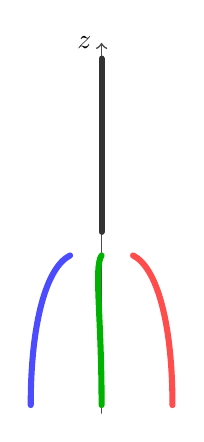
\begin{tikzpicture}[scale=0.5, line cap=round, line join=round]
\tikzset{
    axisline/.style={draw=black!70, line width=0.6pt},
    tube/.style={draw, line width=2.2pt, rounded corners=2pt},
    vline/.style={draw, line width=1.2pt},
    labelbox/.style={fill=white, draw=black!20, rounded corners=2pt, inner sep=3pt}
}
\draw[axisline, ->] (0,-5.2) -- (0,4.2) node[left] {$z$};
\draw[tube, blue!70]
(-1.8,-5.0) .. controls + (0,2.1) and +(-0.6,-0.3) .. (-0.8,-1.2);
\draw[tube, green!70!black]
(0.0,-5.0) .. controls + (0,2.3) and +(-0.2,-0.3) .. (0.0,-1.2);
\draw[tube, red!70]
(1.8,-5.0) .. controls + (0,2.1) and +(0.6,-0.3) .. (0.8,-1.2);
\draw[tube, black!80]
(0.0,-0.6) .. controls +(0,0.9) and +(0,-0.9) .. (0.0,3.8);
\end{tikzpicture}
